% This is text associated with the open textbook "Open Electromagnetics"
% See immediately below for author, date
% This work is licensed under the Creative Commons Attribution-ShareAlike 4.0 International License. (CC BY-SA 4.0) 
% To view a copy of the license, visit http://creativecommons.org/licenses/by-sa/4.0/

%ORB TITLE Voltage Reflection Coefficient
%ORB AUTHOR 0        # S.W. Ellingson, Virginia Tech (ellingson@vt.edu)
%ORB DATE 20180802   # yyyymmdd
%ORB ABSTRACT Voltage reflection coefficient for a lossless transmission line

\label{m0084_Voltage_Reflection_Coefficient} % <-- Must match name of this file and module directory name.  Don't mess with this!
\index{reflection coefficient|(}
\index{voltage reflection coefficient|see{reflection coefficient}}

We now consider the scenario shown in Figure~\ref{m0084_fWaveIncidentOnZL}. 
Here a wave arriving from the left along a lossless transmission line having characteristic impedance $Z_0$ arrives at a termination located at $z=0$.
The impedance looking into the termination is $Z_L$, which may be real-, imaginary-, or complex-valued.
The questions are: Under what circumstances is a reflection -- i.e., a leftward traveling wave -- expected, and what precisely is that wave?
%
\begin{figure}[b!]
\begin{center}
\pdftooltip{{  % note double braces
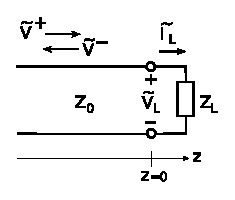
\includegraphics[width=2in]{modules/m0084_fWaveIncidentOnZL.eps}
}}{A lossless transmission line with a wave arriving from the left and with reflected wave traveling to the left. The transmission line is open on the left side with a load on the right side. The current is shown going through the load clockwise.}
\end{center} 
\caption{\label{m0084_fWaveIncidentOnZL}A wave arriving from the left incident on a termination located at $z=0$.}
\end{figure}

The potential and current of the incident wave are related by the constant value of $Z_0$.
Similarly, the potential and current of the reflected wave are related by $Z_0$. 
Therefore, it suffices to consider \emph{either} potential or current.  
Choosing potential, we may express the incident wave as 
%
\begin{equation}
\widetilde{V}^+(z) = V_0^+ e^{-j\beta z}
\end{equation} 
%
where $V_0^+$ is determined by the source of the wave, and so is effectively a ``given.''
Any reflected wave must have the form
%
\begin{equation}
\widetilde{V}^-(z) = V_0^- e^{+j\beta z}
\end{equation} 
%
Therefore, the problem is solved by determining the value of $V_0^-$ given $V_0^+$, $Z_0$, and $Z_L$.

Considering the situation at $z=0$, note that by definition we have
%
\begin{equation}
Z_L \triangleq \frac{\widetilde{V}_L}{\widetilde{I}_L}
\label{m0084_eZL}
\end{equation}
%
where $\widetilde{V}_L$ and $\widetilde{I}_L$ are the potential across and current through the termination, respectively.
Also, the potential and current on either side of the $z=0$ interface must be equal. Thus,
%
\begin{flalign}
\widetilde{V}^+(0) + \widetilde{V}^-(0) & = \widetilde{V}_L \label{m0084_eV1} \\
\widetilde{I}^+(0) + \widetilde{I}^-(0) & = \widetilde{I}_L \label{m0084_eI1}
\end{flalign}
%
where $\widetilde{I}^+(z)$ and $\widetilde{I}^-(z)$ are the currents associated with $\widetilde{V}^+(z)$ and $\widetilde{V}^-(z)$, respectively. 
%
Since the voltage and current are related by $Z_0$, Equation~\ref{m0084_eI1} may be rewritten as follows:
%
\begin{equation}
\frac{\widetilde{V}^+(0)}{Z_0} - \frac{\widetilde{V}^-(0)}{Z_0} = \widetilde{I}_L \label{m0084_eI2}
\end{equation}

Evaluating the left sides of Equations~\ref{m0084_eV1} and \ref{m0084_eI2} at $z=0$, we find:
%
\begin{flalign}
V_0^+ + V_0^- &= \widetilde{V}_L \\
\frac{V_0^+}{Z_0} - \frac{V_0^-}{Z_0} &= \widetilde{I}_L
\end{flalign}
%
Substituting these expressions into Equation~\ref{m0084_eZL} we obtain:
%
\begin{equation}
Z_L = \frac{V_0^+ + V_0^-}{V_0^+/Z_0 - V_0^-/Z_0}
\end{equation}
%
Solving for $V_0^-$ we obtain
%
\begin{equation}
V_0^- = \frac{Z_L-Z_0}{Z_L+Z_0}~V_0^+
\end{equation}
%
Thus, the answer to the question posed earlier is that 
%
\begin{equation}
V_0^- = \Gamma V_0^+ ~~\mbox{, where}
\end{equation}
%
\begin{equation}
\boxed{
\Gamma \triangleq \frac{Z_L-Z_0}{Z_L+Z_0}
}
\label{m0084_eGamma}
\end{equation}

The quantity $\Gamma$ is known as the \emph{voltage reflection coefficient}.
Note that when $Z_L=Z_0$, $\Gamma=0$ and therefore $V_0^-=0$. 
In other words, 
%
%ORB HIGHLIGHT
\begin{mdframed}[backgroundcolor=yellow!20,nobreak=true] 
If the terminating impedance is equal to the characteristic impedance 
\index{characteristic impedance}
of the transmission line, then there is no reflection. 
\end{mdframed}
%
If, on the other hand, $Z_L \neq Z_0$, then $\left|\Gamma\right|>0$, $V_0^-= \Gamma V_0^+$, and a leftward-traveling reflected wave exists.

Since $Z_L$ may be real-, imaginary-, or complex-valued, $\Gamma$ too may be real-, imaginary-, or complex-valued. 
Therefore, $V_0^-$ may be different from $V_0^+$ in magnitude, sign, or phase.  

Note also that $\Gamma$ is \emph{not} the ratio of $I_0^-$ to $I_0^+$.  
The ratio of the \emph{current} coefficients is actually $-\Gamma$.
It is quite simple to show this with a simple modification to the above procedure and is left as an exercise for the student.

Summarizing:
%
%ORB HIGHLIGHT
\begin{mdframed}[backgroundcolor=yellow!20,nobreak=true] 
The voltage reflection coefficient 
\index{reflection coefficient!definition}
$\Gamma$, given by Equation~\ref{m0084_eGamma}, determines the magnitude and phase of the reflected wave given the incident wave, the characteristic impedance of the transmission line, and the terminating impedance. 
\end{mdframed}

\index{reflection coefficient|)}
